\thispagestyle{fancy}


\section{Metallorganische Gasphasenepitaxie von AlGaN}

Die Metallorganische Gasphasenepitaxie (engl.: matalorganic vapor phase epitaxy, kurz MOVPE) ist die gängigste Methode um epitaktische Schichten hoher Qualität in ebenfalls hoher Quantität zu wachsen. Es werden gasförmige Ausgangsstoffe in den Reaktor geleitet und dort bei hohen Temperaturen pyrolytisch zerlegt. Ein Teil der derartig zerlegten Ausgangsstoffe adsorbiert auf der Oberfläche des verwendeten Substrates und kristallisiert dort schließlich als Epitaxieschicht. 

\section{Substrat}

In der Epitaxie beruhen viele Eigenschaften der aufgewachsenen Schichten auf dem dazu verwendeten Substrat. So sind Gitterfehlanpassung, Defektdichte und die Morphologie wichtige Eigenschaften, die durch das Substrat maßgeblich beeinflusst werden. Für AlGaN kann theoretisch auf verschiedene Substrate zurückgegriffen werden und die Vermutung direkt AlGaN basierte Substrate zu verwenden liegt nahe. Dies scheitert allerdings an der besonders hohen Schwierigkeit bei der Herstellung. Daraus resultierend weisen diese Substrate hohe Defektdichten auf und sind mit sehr hohen Kosten verbunden. Weiterhin ist GaN/Saphir oder GaN als Volumenkristall kommerziell in großen Mengen und hoher Qualität erhältlich, aber aufgrund der Gitterfehlanpassung zwischen AlN und GaN reißen AlGaN-Schichten mit hohem Aluminiumgehalt auf GaN wegen Relaxation \cite{problem} wie in Abbildung \ref{fig:wachstum} dargestellt.
\begin{figure}[h]
    \centering
    \begin{minipage}[t]{1\linewidth}
    \centering
    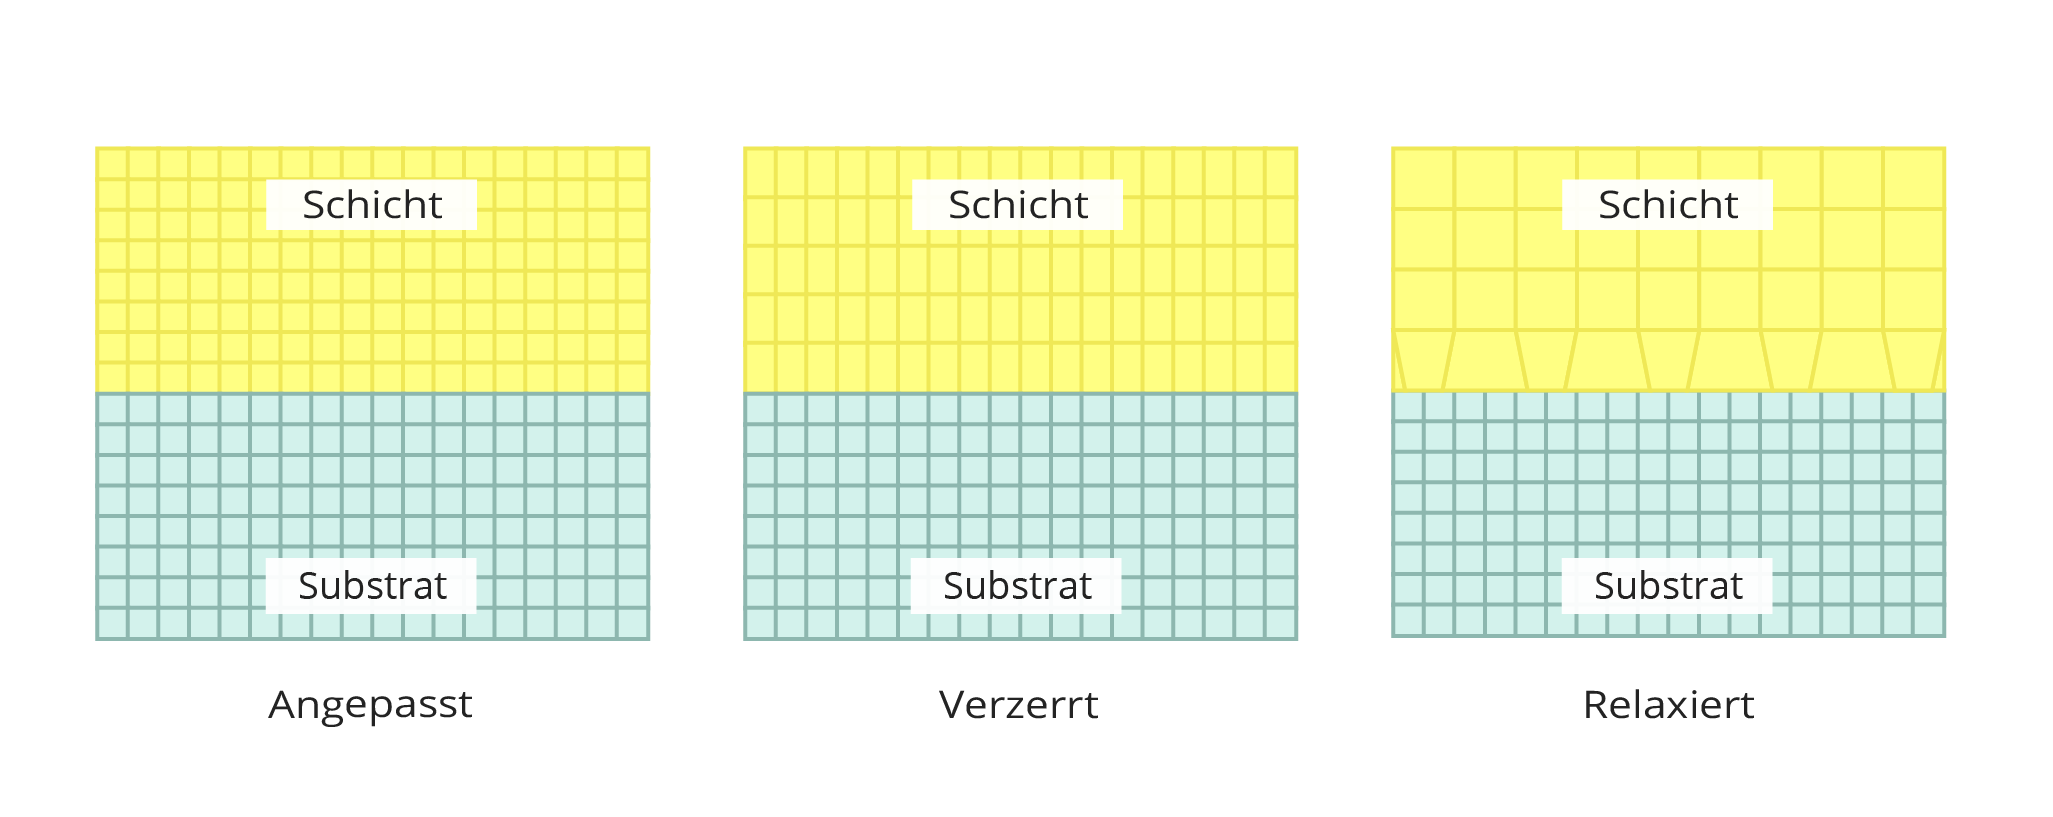
\includegraphics[width=1\linewidth]{Bilder/wachstumsarten.png}
    \end{minipage}% <- sonst wird hier ein Leerzeichen eingefügt
    \caption{Verfahren zum epitaktisch lateralen Wachstum.}
     \label{fig:wachstum}
\end{figure} 
Ein weiterer ungewollter Effekt ist die Absorption von UV-Strahlung ($\lambda \leq 365 \thinspace nm$) im GaN und erlaubt damit keine Verwendung im UV-B und UV-C-Bereich. Daher werden UV-B- und UV-C LEDs und Laserdioden hauptsächlich auf AlN/Saphir oder auf AlN als Volumenkristall gewachsen. Der AlN Volumenkristall weist dabei die kleinste Defektdichte mit $<10^4 \thinspace cm^2$ auf. Jedoch ist die Ausbeute der AlN Substrate zeitaufwendig und teuer. Daher wird für Forschungszwecke auf AlN/Saphir zurückgegriffen und dabei aber eine hohe Defektdichte in Kauf genommen. Defekte entstehen dabei im Kristall wegen der hohen Gitterfehlanpassung an der Grenzfläche zwischen AlN und Spahir \cite{pohl}. Diese Defekte ziehen sich dabei durch die darauffolgenden aufgewachsenen Schichten. Diese sog. Schraubenversetzungen (engl.: threading dislocation) haben einen wesentlichen Einfluss auf die IQE, wie in Abbildung \ref{fig:IQEthreadingdisl} erkennbar. 
%
\begin{figure}[h]
\centering
\begin{minipage}[t]{1\linewidth}
\centering
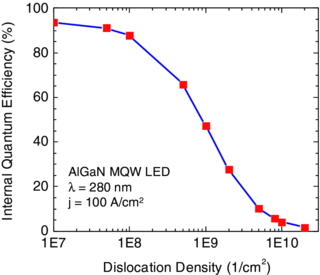
\includegraphics[width=0.5\linewidth]{Bilder/IQEthreadingdisl.PNG}
\end{minipage}% <- sonst wird hier ein Leerzeichen eingefügt
\caption{Simulation der IQE einer LED in Abhängigkeit der Versetzungsdichte für einen AlGaN-MQW mit einer Wellenlänge von $280 \thinspace nm$ \cite{0268-1242-26-1-014036}.}
 \label{fig:IQEthreadingdisl}
\end{figure}
\noindent
%
Sie agieren im Kristall als nicht-radiative Rekombinationszentren (engl.: nonradiative recombination center, kurz NRC) und bestimmen somit den Anteil nichtstrahlender Rekombinationsprozesse an der Gesamtheit aller Rekombinationsprozesse. Mit steigender Versetzungsdichte sinkt die IQE der Leuchtdiode und im Bereich zwischen $1\cdot 10^10 \thinspace cm^{-2}$ und $1\cdot 10^8 \thinspace cm^{-2}$ ist eine erhebliche Steigerung zu beobachten. Mittels XRD und TEM wurde gezeigt, dass die Heteroepitaxie von AlN Schichten auf Saphir zu einer Defektdichte von bis zu $2\cdot 10^{10} \thinspace cm^{-2}$ führt \cite{zeimeru}.

\section{Defektreduktion durch ELO/AlN-Saphir}

Um die hohe Defektdichte des planaeren AlN/Saphir Substrates zu verringern, ist der übliche Ansatz das sog. epitaktisch laterale Überwachsen (engl.: epitaxial lateral overgrowth) oder kurz ELO. Diese Substrate wurden für alle in dieser Arbeit untersuchten Proben verwendet. 
\begin{figure}[h]
    \centering
    \begin{minipage}[t]{1\linewidth}
    \centering
    \includegraphics[width=1\linewidth]{Bilder/elostrukturierung.png}
    \end{minipage}% <- sonst wird hier ein Leerzeichen eingefügt
    \caption{Verfahren zum epitaktisch lateralen Wachstum.}
     \label{fig:IQEthreadingdisl}
\end{figure}
\noindent
Als Grundlage für ELO dient ein planares AlN/Saphir Substrat. Dieses wird strukturiert indem ein Streifenmuster mit einem periodischen Abstand von $3.5 \thinspace \mu m$ reingeätzt wird. Ein weiterer Epitaxie-Schritt mit AlN führt schließlich zum lateralen Überwachsen der Stege an den geätzten Gräben (eng.: voids).
Das Material koalesziert nach einer bestimmten Dicke und bildet schließlich wieder eine bewachsbare Oberfläche. Dabei kommt es zum Auftreten verschiedener Mechanismen wie Verspannungsabbau und gegenseitig auslöschenden Versetzungen. So ist eine Defektdichte ($\leq 5 \cdot 10^8 \thinspace cm^{-2}$) erreichbar \cite{zeimeru} \cite{MOGILATENKO2014222} \cite{vkueller} \cite{IMURA2007257}. Für eine detaillierte Erklärung sei auf die Doktorarbeit von Viola Küller verwiesen \cite{vkueller}.